\section{Multi-Comparison}

\subsection{Introduction}
As our intended goal of this project is to locate the ROI (Region of Interest) in a brain a
ccording to this mixed gamble task, the significant issue is the specification of an appropr
iate threshold for statistical maps. Therefore, we are interested in multi-comparison acros
s subjects. In the previous analysis on single subject, we were able to locate the generall
y activated voxels. With these data, we attempted to find out the general pattern in each vo
xel of brains across 16 subjects. 

\subsection{Methods}
As our intended goal of this project is to locate the ROI (Region of Interest) in a brain 
according to this mixed gamble task, the significant issue is the specification of an appropr
iate threshold for statistical maps. Therefore, we are interested in multi-comparison across 
subjects. In the previous analysis on single subject, we were able to locate the generally ac
tivated voxels. With these data, we attempted to find out the general pattern in voxels of br
ains across 16 subjects. 

To multi-compare, we chose to explore on filtered data set (shape: 91*109 * 91) since original
 data set is not normalized in terms of voxel location. Applying our general linear modeling o
 n each subject as above, we first collected all beta values for each voxel across time course
  of each subject. Now, we have beta values of shape of (91, 109, 91) for each of 16 subjects.
   We compare on each single voxel across subjects. To do this, We have total 4 steps.

\begin{itemize}
\item Calculate average of beta value on a single voxel across 16 subjects. Do this for whole v
oxels.
\item Calculate standard deviation of beta value on a single voxel across 16 subjects. Do this 
for whole voxels. 
\item Calculate T-statistics of beta value on a single voxel across 16 subjects. Do this for who
le voxels.
\[ 
  t-statistics = \dfrac{mean}{\dfrac{SE(mean)}{\sqrt{n}}}
\]

\item Calculate P-value of beta value on a single voxel across 16 subjects. Do this for whole vo
xels. 
\end{itemize}

For the 4th step, we have an issue of false positives: since we're executing 91\*109\*91 number
 of hypothesis testing, note that an error probability of p value = 0.05 means that if we would 
 repeat the same test 1000 times and assume that there is no effect of the experiment, we would
  wrongly reject or accept the null or alternative hypothesis on average. Therefore, we dec
  ided to strengthen our p-value threshold with Bon-ferroni correction: our new p-value thresho
  ld is 0.
  05/(91\*109\*91)

\begin{figure}[H] 
\centering 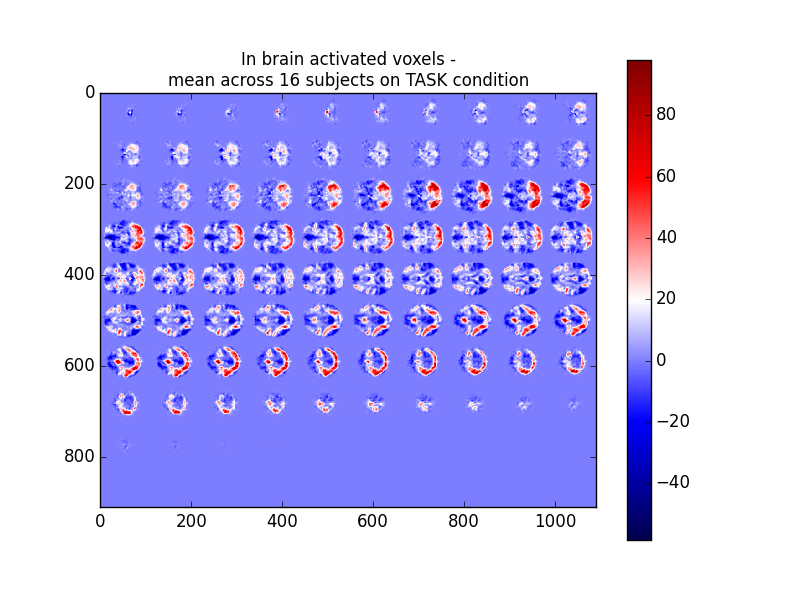
\includegraphics[scale=0.5]{../fig/multi_beta/mean_task.png}	 
\caption{Mean beta values on each voxel across 16 subjects on TASK condition}
\end{figure} 


\subsection {Results}
As the image of mean of beta values on each voxel across all subjects on task condition indicat
es, we are able to classify which portion of brain is in general activated due to this experime
nt. However, there should be fluctuation over different subjects. To identify this, standard de
viation is also shown. As the image in the appendix illustrates, fluctuation occurs on similar r
egions because each subject's hemodynamic response degree must be different. We found out that th
e t-statistics in general are not significant enough; therefore, we could not elaborately indicat
e the specific portion of brain related to the mixed gamble task. However, t-statistics and p
-value of voxels over a brain well correspond to each other.





